\documentclass[9.5pt,a4paper]{article}
\usepackage[margin=1.2cm,headheight=1.2cm,headsep=6pt,footskip=12pt]{geometry}
\usepackage{graphicx}
\usepackage{fancyhdr}
\usepackage{booktabs}
\usepackage{tabularx}
\usepackage{array}
\usepackage{amsmath,amssymb}
\usepackage{microtype}
\usepackage{multirow}
\usepackage{enumitem}

\pagestyle{fancy}
\fancyhf{}
\fancyhead[L]{%
  \begin{tabular}{@{}c@{\hspace{6pt}}l@{}}
    \multirow{2}{*}{
\includegraphics[width=0.85cm]{fast_logo.png}} & \textbf{FAST NUCES}\\
    & {\footnotesize Computer Science}
  \end{tabular}%
}
\fancyhead[R]{%
  \begin{tabular}{@{}r@{}}
    \textbf{25i-0817}\\
    \textbf{Ahmad Ali}
  \end{tabular}%
}
\fancyfoot[L]{\footnotesize FAST NUCES Islamabad}
\fancyfoot[C]{\footnotesize CS2001 Data Structures Phase 1 Report}
\fancyfoot[R]{\footnotesize Page \thepage\ of 3}
\renewcommand{\headrulewidth}{0.4pt}
\renewcommand{\footrulewidth}{0.4pt}

\begin{document}

% =========================================================================
% PAGE 1: COVER AND SELECTED ARCHITECTURE (I SELECT / WHY)
% =========================================================================
\thispagestyle{empty}

\begin{center}
    
\includegraphics[width=2.0cm]{fast_logo.png}\\[4pt]
    {\LARGE \textbf{National University of Computer and Emerging Sciences}}\\[6pt]
    {\huge \textbf{DSA Assignment 2 Phase 1 Report}}\\[6pt]
    \rule{0.88\textwidth}{0.6pt}\\[5pt]
    {\large \textbf{Student Name: Ahmad Ali} \qquad \textbf{Roll Number: 25i-0817} \qquad \textbf{Section: BS CS E}}\\[3pt]
    \rule{0.88\textwidth}{0.6pt}\\[10pt]
    {\Large \textbf{Selected Data Structures and Justifications}}
\end{center}

\vspace{0.1cm}
\begin{itemize}[noitemsep,topsep=1pt,parsep=3pt,partopsep=0pt]
    \item \textbf{Stack Representation}
    
    \textbf{I select dynamic array} because:
    \begin{enumerate}[noitemsep,topsep=1pt,parsep=1pt]
        \item It stores elements in continuous memory for instant access.
        \item Push and pop run in strict O(1) time without pointer overhead.
        \item It dynamically doubles memory when full so no operation fails.
    \end{enumerate}

    \item \textbf{Queue Representation}
    
    \textbf{I select circular array} because:
    \begin{enumerate}[noitemsep,topsep=1pt,parsep=1pt]
        \item It connects front and rear pointers using modulo arithmetic.
        \item Add and delete run in O(1) time without moving or shifting elements.
        \item It enforces bounded capacity to protect memory from uncontrolled growth.
    \end{enumerate}

    \item \textbf{Empty Queue versus Full Queue Identification}
    
    \textbf{I select dedicated count variable} because:
    \begin{enumerate}[noitemsep,topsep=1pt,parsep=1pt]
        \item It directly tracks the active element count at any point.
        \item It tells full from empty without wasting a reserved slot in the array.
        \item It provides an instant O(1) answer for queue size queries.
    \end{enumerate}

    \item \textbf{Bounded Pipeline Policy}
    
    \textbf{I select reject new jobs when full} because:
    \begin{enumerate}[noitemsep,topsep=1pt,parsep=1pt]
        \item It stops memory overflow when maximum queue capacity is reached.
        \item It prompts the user to process pending tasks before adding new ones.
        \item It maintains application stability under heavy edit requests.
    \end{enumerate}

    \item \textbf{Pipeline Job Cancellation Policy}
    
    \textbf{I select in place cancellation marker flag} because:
    \begin{enumerate}[noitemsep,topsep=1pt,parsep=1pt]
        \item It flags the job as cancelled without shifting other elements.
        \item It avoids rebuilding or reordering the queue array.
        \item The pipeline safely skips the task when it reaches the front during execution.
    \end{enumerate}

    \item \textbf{Pending Jobs with Undo and Redo Policy}
    
    \textbf{I select queued execution when pipeline is active} because:
    \begin{enumerate}[noitemsep,topsep=1pt,parsep=1pt]
        \item It preserves the exact chronological order of editing actions.
        \item It ensures an undo operates on the image only after earlier queued jobs finish.
        \item It runs immediately whenever the pipeline queue is empty.
    \end{enumerate}

    \item \textbf{Bucket Fill Traversal}
    
    \textbf{I select non recursive Stack fill and Queue fill} because:
    \begin{enumerate}[noitemsep,topsep=1pt,parsep=1pt]
        \item Stack fill explores deep neighbor branches along one path first.
        \item Queue fill spreads outward evenly in concentric radial waves.
        \item Explicit data structures prevent system call stack overflow on large images.
    \end{enumerate}

    \item \textbf{History Management Engine}
    
    \textbf{I select dual stacks with deep copy snapshots} because:
    \begin{enumerate}[noitemsep,topsep=1pt,parsep=1pt]
        \item It isolates undo history from redo history cleanly.
        \item Any fresh edit immediately clears the redo stack to keep history linear.
        \item Full matrix snapshots guarantee bit for bit image recovery upon undo.
    \end{enumerate}
\end{itemize}

\clearpage

% =========================================================================
% PAGE 2: COMPLEXITY TABLE WITH ONE-LINE REASONS ("I USE ...")
% =========================================================================

\begin{center}
    {\Large \textbf{Operation Complexity and Analysis}}
\end{center}

\vspace{0.08cm}
\begin{table}[h!]
\centering
\fontsize{7.5pt}{9.2pt}\selectfont
\begin{tabularx}{\textwidth}{l c c X}
\toprule
\textbf{Operation Name} & \textbf{Time} & \textbf{Space} & \textbf{Reason} \\
\midrule
Load Image & $\mathcal{O}(W \times H)$ & $\mathcal{O}(1)$ & I use binary stream reading to parse image header and stream pixels directly into grid. \\
\addlinespace[1pt]
Crop Image & $\mathcal{O}(W' \times H')$ & $\mathcal{O}(W' \times H')$ & I use nested loops to copy pixels strictly within the selected crop bounding box. \\
\addlinespace[1pt]
Rotate 90 and 270 deg & $\mathcal{O}(W \times H)$ & $\mathcal{O}(W \times H)$ & I use coordinate transposition which maps source rows into target columns. \\
\addlinespace[1pt]
Rotate 180 deg & $\mathcal{O}(W \times H)$ & $\mathcal{O}(1)$ & I use symmetric in place pointer swapping between opposite halves of the image grid. \\
\addlinespace[1pt]
Horizontal Flip & $\mathcal{O}(W \times H)$ & $\mathcal{O}(1)$ & I use in place swapping of symmetric column pixels along each row. \\
\addlinespace[1pt]
Vertical Flip & $\mathcal{O}(H)$ & $\mathcal{O}(1)$ & I use direct row pointer swaps which avoids touching individual pixel data. \\
\addlinespace[1pt]
Brightness Adjustment & $\mathcal{O}(W \times H)$ & $\mathcal{O}(1)$ & I use direct arithmetic addition and clamp every value between 0 and 255. \\
\addlinespace[1pt]
Grayscale Conversion & $\mathcal{O}(W \times H)$ & $\mathcal{O}(1)$ & I use fixed point luminance weighting to compute average intensity per pixel. \\
\addlinespace[1pt]
Bilinear Resize & $\mathcal{O}(W' \times H')$ & $\mathcal{O}(W' \times H')$ & I use four point weighted interpolation for each target dimension pixel. \\
\addlinespace[1pt]
Box Blur ($3 \times 3$) & $\mathcal{O}(W \times H)$ & $\mathcal{O}(W \times H)$ & I use standard matrix kernel where 9 neighbor sums take O(1) time per pixel. \\
\addlinespace[1pt]
Bucket Fill (Stack) & $\mathcal{O}(W \times H)$ & $\mathcal{O}(W \times H)$ & I use an explicit stack to visit every connected matching pixel once. \\
\addlinespace[1pt]
Bucket Fill (Queue) & $\mathcal{O}(W \times H)$ & $\mathcal{O}(W \times H)$ & I use a circular queue to expand outward layer by layer in level order. \\
\addlinespace[1pt]
Stack Push, Pop, Top & $\mathcal{O}(1)$ & $\mathcal{O}(1)$ & I use direct indexing at the stack top position without moving elements. \\
\addlinespace[1pt]
Queue Add, Delete, Front & $\mathcal{O}(1)$ & $\mathcal{O}(1)$ & I use circular modulo arithmetic to advance front and rear pointers instantly. \\
\addlinespace[1pt]
Undo and Redo Operation & $\mathcal{O}(W \times H)$ & $\mathcal{O}(W \times H)$ & I use deep copy restoration to pop snapshot state from stack to canvas. \\
\bottomrule
\end{tabularx}
\end{table}

\vspace{0.1cm}
\begin{center}
    {\large \textbf{Core Operational Guarantees}}
\end{center}
\begin{itemize}[noitemsep,topsep=1.5pt,parsep=1pt]
    \item \textbf{Strict Zero Shifting:} The circular queue never shifts elements upon \texttt{deleteQueue()}. Pointers advance via $(rear + 1) \pmod{capacity}$ and $(front + 1) \pmod{capacity}$.
    \item \textbf{Stack Safety and Growth:} The stack dynamically doubles memory when full, ensuring no push fails, and checks empty status to prevent underflow crashes.
    \item \textbf{Four Connectivity Rule:} Bucket fill inspects only up, down, left, and right neighbors. Diagonal pixels are never accessed.
    \item \textbf{Identical Output Proof:} Both Stack fill and Queue fill produce bit for bit identical output images for identical seed coordinates and replacement colors.
\end{itemize}

\clearpage

% =========================================================================
% PAGE 3: TEST SUITE RESULTS AND VISUAL PROOF
% =========================================================================

\begin{center}
    {\Large \textbf{Testing Evidence and Verification Results}}
\end{center}

\vspace{0.08cm}
\begin{table}[h!]
\centering
\fontsize{7.8pt}{9.8pt}\selectfont
\begin{tabularx}{\textwidth}{l X c}
\toprule
\textbf{Component Tested} & \textbf{Cases Verified} & \textbf{Result} \\
\midrule
\textbf{Stack (stackType)} & Pop and top on empty stack; 1000 item capacity; repeated push pop cycles; stack reset; deep copy constructor and assignment. & \textbf{PASS} \\
\addlinespace[1.5pt]
\textbf{Queue (queueType)} & Delete and front on empty queue; full queue rejection; circular wrap around; drain and re add; deep copy constructor. & \textbf{PASS} \\
\addlinespace[1.5pt]
\textbf{Undo and Redo Engine} & Multiple consecutive undos; multiple consecutive redos; clearing redo stack after new action; bit for bit image recovery. & \textbf{PASS} \\
\addlinespace[1.5pt]
\textbf{Bucket Fill Engine} & Single pixel fill; full image fill; irregular boundary fill; disconnected regions; identical Stack and Queue outputs; same color immediate exit. & \textbf{PASS} \\
\addlinespace[1.5pt]
\textbf{Processing Pipeline} & Bounded queue rejection; process next and all jobs; in place job cancellation without shifting; queue clearing. & \textbf{PASS} \\
\bottomrule
\end{tabularx}
\end{table}

\vspace{0.1cm}
\begin{center}
    {\large \textbf{Visual Verification: Bucket Fill and Test Suite Execution}}\\[5pt]
    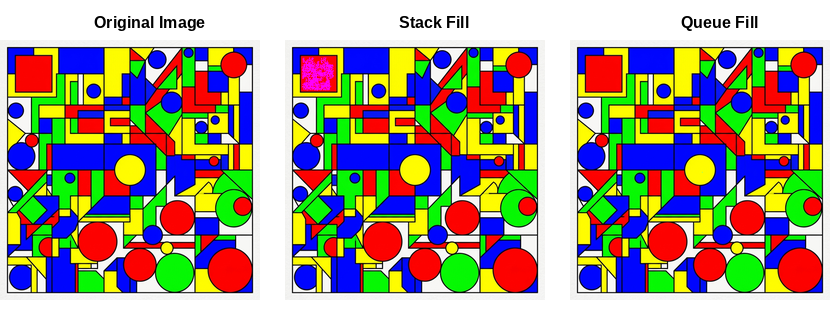
\includegraphics[width=0.88\textwidth,height=2.85cm,keepaspectratio]{bucket_fill_comparison.png}\\[3pt]
    {\footnotesize \textbf{Figure 1:} Side by side visual proof: Stack fill (middle) and Queue fill (right) yield identical results.}\\[6pt]
    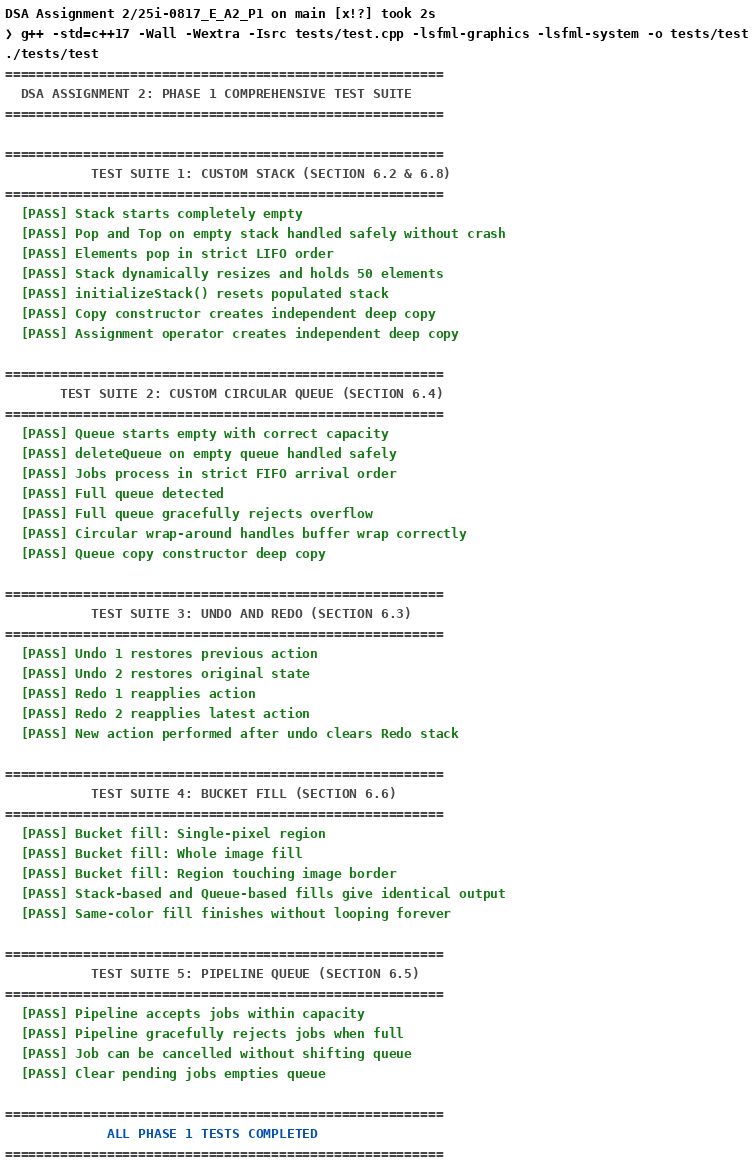
\includegraphics[width=0.88\textwidth,height=4.5cm,keepaspectratio]{test_results_trimmed.png}\\[3pt]
    {\footnotesize \textbf{Figure 2:} Automated test suite output verifying 100 percent pass across all required edge cases.}
\end{center}

\end{document}
